%% Creator: Inkscape inkscape 0.48.0, www.inkscape.org
%% PDF/EPS/PS + LaTeX output extension by Johan Engelen, 2010
%% Accompanies image file 'picLF2+LF4.eps' (pdf, eps, ps)
%%
%% To include the image in your LaTeX document, write
%%   \input{<filename>.pdf_tex}
%%  instead of
%%   \includegraphics{<filename>.pdf}
%% To scale the image, write
%%   \def\svgwidth{<desired width>}
%%   \input{<filename>.pdf_tex}
%%  instead of
%%   \includegraphics[width=<desired width>]{<filename>.pdf}
%%
%% Images with a different path to the parent latex file can
%% be accessed with the `import' package (which may need to be
%% installed) using
%%   \usepackage{import}
%% in the preamble, and then including the image with
%%   \import{<path to file>}{<filename>.pdf_tex}
%% Alternatively, one can specify
%%   \graphicspath{{<path to file>/}}
%% 
%% For more information, please see info/svg-inkscape on CTAN:
%%   http://tug.ctan.org/tex-archive/info/svg-inkscape

\begingroup
  \makeatletter
  \providecommand\color[2][]{%
    \errmessage{(Inkscape) Color is used for the text in Inkscape, but the package 'color.sty' is not loaded}
    \renewcommand\color[2][]{}%
  }
  \providecommand\transparent[1]{%
    \errmessage{(Inkscape) Transparency is used (non-zero) for the text in Inkscape, but the package 'transparent.sty' is not loaded}
    \renewcommand\transparent[1]{}%
  }
  \providecommand\rotatebox[2]{#2}
  \ifx\svgwidth\undefined
    \setlength{\unitlength}{207.0671875pt}
  \else
    \setlength{\unitlength}{\svgwidth}
  \fi
  \global\let\svgwidth\undefined
  \makeatother
  \begin{picture}(1,1.12792072)%
    \put(0,0){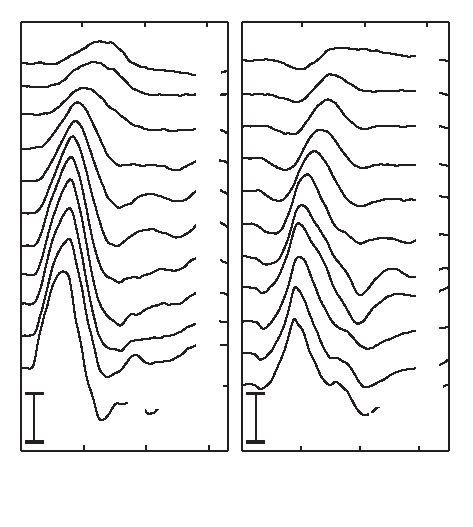
\includegraphics[width=\unitlength]{pics/picLF2+LF4.eps}}%
    \put(0,0.09){\color[rgb]{0,0,0}\makebox(0,0)[lb]{\smash{$0$}}}%
    \put(0.138,0.09){\color[rgb]{0,0,0}\makebox(0,0)[lb]{\smash{$1$}}}%
    \put(0.28,0.09){\color[rgb]{0,0,0}\makebox(0,0)[lb]{\smash{$2$}}}%
    \put(0.426,0.09){\color[rgb]{0,0,0}\makebox(0,0)[lb]{\smash{$3$}}}%
    \put(0.5,0.09){\color[rgb]{0,0,0}\makebox(0,0)[lb]{\smash{$0$}}}%
    \put(0.636,0.09){\color[rgb]{0,0,0}\makebox(0,0)[lb]{\smash{$1$}}}%
    \put(0.77,0.09){\color[rgb]{0,0,0}\makebox(0,0)[lb]{\smash{$2$}}}%
    \put(0.904,0.09){\color[rgb]{0,0,0}\makebox(0,0)[lb]{\smash{$3$}}}%
    \put(0.67,0.006){\color[rgb]{0,0,0}\makebox(0,0)[lb]{\smash{$t$\,(мкс)}}}%
    \put(0.18,0.006){\color[rgb]{0,0,0}\makebox(0,0)[lb]{\smash{$t$\,(мкс)}}}%
    \put(0.07,0.16){\color[rgb]{0,0,0}\makebox(0,0)[lb]{\smash{$0.2$\,мГc}}}%
    \put(0.02,1.06){\color[rgb]{0,0,0}\makebox(0,0)[lb]{\smash{$(а)$}}}%
    \put(0.52,1.06){\color[rgb]{0,0,0}\makebox(0,0)[lb]{\smash{$(б)$}}}%
    \put(0.41,0.98){\color[rgb]{0,0,0}\makebox(0,0)[lb]{\smash{$50$}}}%
    \put(0.41,0.93){\color[rgb]{0,0,0}\makebox(0,0)[lb]{\smash{$46$}}}%
    \put(0.41,0.85){\color[rgb]{0,0,0}\makebox(0,0)[lb]{\smash{$42$}}}%
    \put(0.41,0.78){\color[rgb]{0,0,0}\makebox(0,0)[lb]{\smash{$38$}}}%
    \put(0.41,0.716){\color[rgb]{0,0,0}\makebox(0,0)[lb]{\smash{$34$}}}%
    \put(0.41,0.64){\color[rgb]{0,0,0}\makebox(0,0)[lb]{\smash{$30$}}}%
    \put(0.41,0.56){\color[rgb]{0,0,0}\makebox(0,0)[lb]{\smash{$26$}}}%
    \put(0.41,0.48){\color[rgb]{0,0,0}\makebox(0,0)[lb]{\smash{$22$}}}%
    \put(0.41,0.412){\color[rgb]{0,0,0}\makebox(0,0)[lb]{\smash{$18$}}}%
    \put(0.41,0.35){\color[rgb]{0,0,0}\makebox(0,0)[lb]{\smash{$14$}}}%
    \put(0.27,0.24){\color[rgb]{0,0,0}\makebox(0,0)[lb]{\smash{$r=10$\,см}}}%
    \put(0.57646597,0.16){\color[rgb]{0,0,0}\makebox(0,0)[lb]{\smash{$0.2$\,мГс}}}%
    \put(0.774,0.24){\color[rgb]{0,0,0}\makebox(0,0)[lb]{\smash{$r=10$\,см}}}%
    \put(0.91,0.31){\color[rgb]{0,0,0}\makebox(0,0)[lb]{\smash{$14$}}}%
    \put(0.91,0.39){\color[rgb]{0,0,0}\makebox(0,0)[lb]{\smash{$18$}}}%
    \put(0.91,0.47){\color[rgb]{0,0,0}\makebox(0,0)[lb]{\smash{$22$}}}%
    \put(0.91,0.53){\color[rgb]{0,0,0}\makebox(0,0)[lb]{\smash{$26$}}}%
    \put(0.91,0.61){\color[rgb]{0,0,0}\makebox(0,0)[lb]{\smash{$30$}}}%
    \put(0.91,0.7){\color[rgb]{0,0,0}\makebox(0,0)[lb]{\smash{$34$}}}%
    \put(0.91,0.77){\color[rgb]{0,0,0}\makebox(0,0)[lb]{\smash{$38$}}}%
    \put(0.91,0.86){\color[rgb]{0,0,0}\makebox(0,0)[lb]{\smash{$42$}}}%
    \put(0.91,0.94){\color[rgb]{0,0,0}\makebox(0,0)[lb]{\smash{$46$}}}%
    \put(0.91,1.02){\color[rgb]{0,0,0}\makebox(0,0)[lb]{\smash{50}}}%
  \end{picture}%
\endgroup
